\chapter{Implementation}
\label{chap:Impl}
\section{Programming APIs}

To implement VR applications, we can work directly with the SDK provided from each headset manufacturer, the advantage is that we can interact at a low level with the devices.\\ 
Another way is to use an SDK of a well-defined standard for example OpenVR from Valve or OpenXR from the Khronos group. This allows us to write applications for a target group of devices like 6-DOF supporting headsets without having to deal with different manufacturer SDKs (see Figure \ref{fig:openxr-overview}). On a side note: the X in OpenXR means that the specification is not only used for virtual reality (VR) applications but also for augmented reality (AR) and other technologies (XR) possibly proposed in the future.\\
Lastly, we can work with different engines which will provide with additional features. While classical desktop engines rely on downloading a complete bundled software package for distributing the application, WebXR and WebVR allow us to distribute and run our application via the browser, similar to WebGL.

At the time of writing, the OpenXR and WebXR specification is still relatively new being in its first revision therefore it is not implemented by each headset manufacturer, browser and engine yet. However, these standards are meant to replace the old OpenVR and WebVR in the future.

\begin{figure}[!hbt]
    \centering
    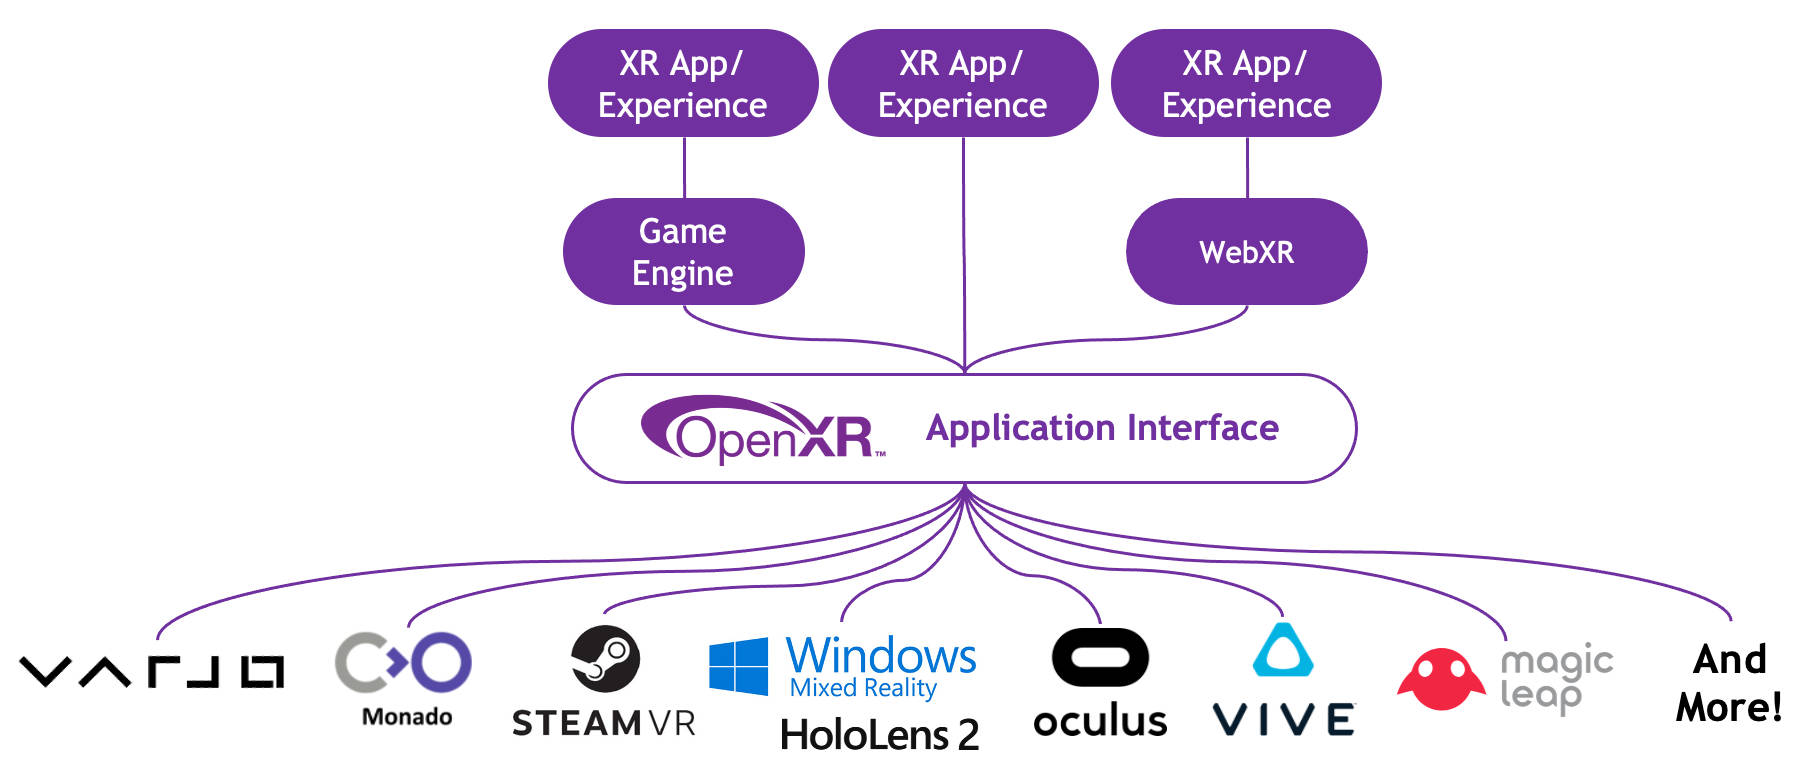
\includegraphics[width=\textwidth]{graphics/openXR-overview.jpg}
    \caption{Overview of the OpenXR API Stack \cite{khronosGroupOpenXR}}
    \label{fig:openxr-overview}
\end{figure}

\section{Prior Publication}
For our implementation we extend the code from a prior publication from Sorger et al. \cite{sorger_immersive_2019}. 
They implemented an immersive visualization for node-link graphs without hierarchical information. Their implementation already contains a common force-based layout, the laser-pointer ray casting technique to select objects, a free flying navigation as well as the animated teleport and lastly the code structure to include the frameworks they use. A screenshot of their work is shown in Figure \ref{fig:priorPublication}.\\
We extend their implementation by adding ability to visualization hierarchical networks as described in Section \ref{chap:proposed-Solution}. To achieve that we had to adapt the layout algorithm, add transparent rendering, adapt some visual rendering aspects, change the target position for the animated teleport, change the controller button mappings, implement the link filtering technique, add automatic/manual scaling of the virtual scene and automatic/manual adaption of the free flying speed.
This process is described in detail in this chapter.

\begin{figure}[!hbt]
    \centering
    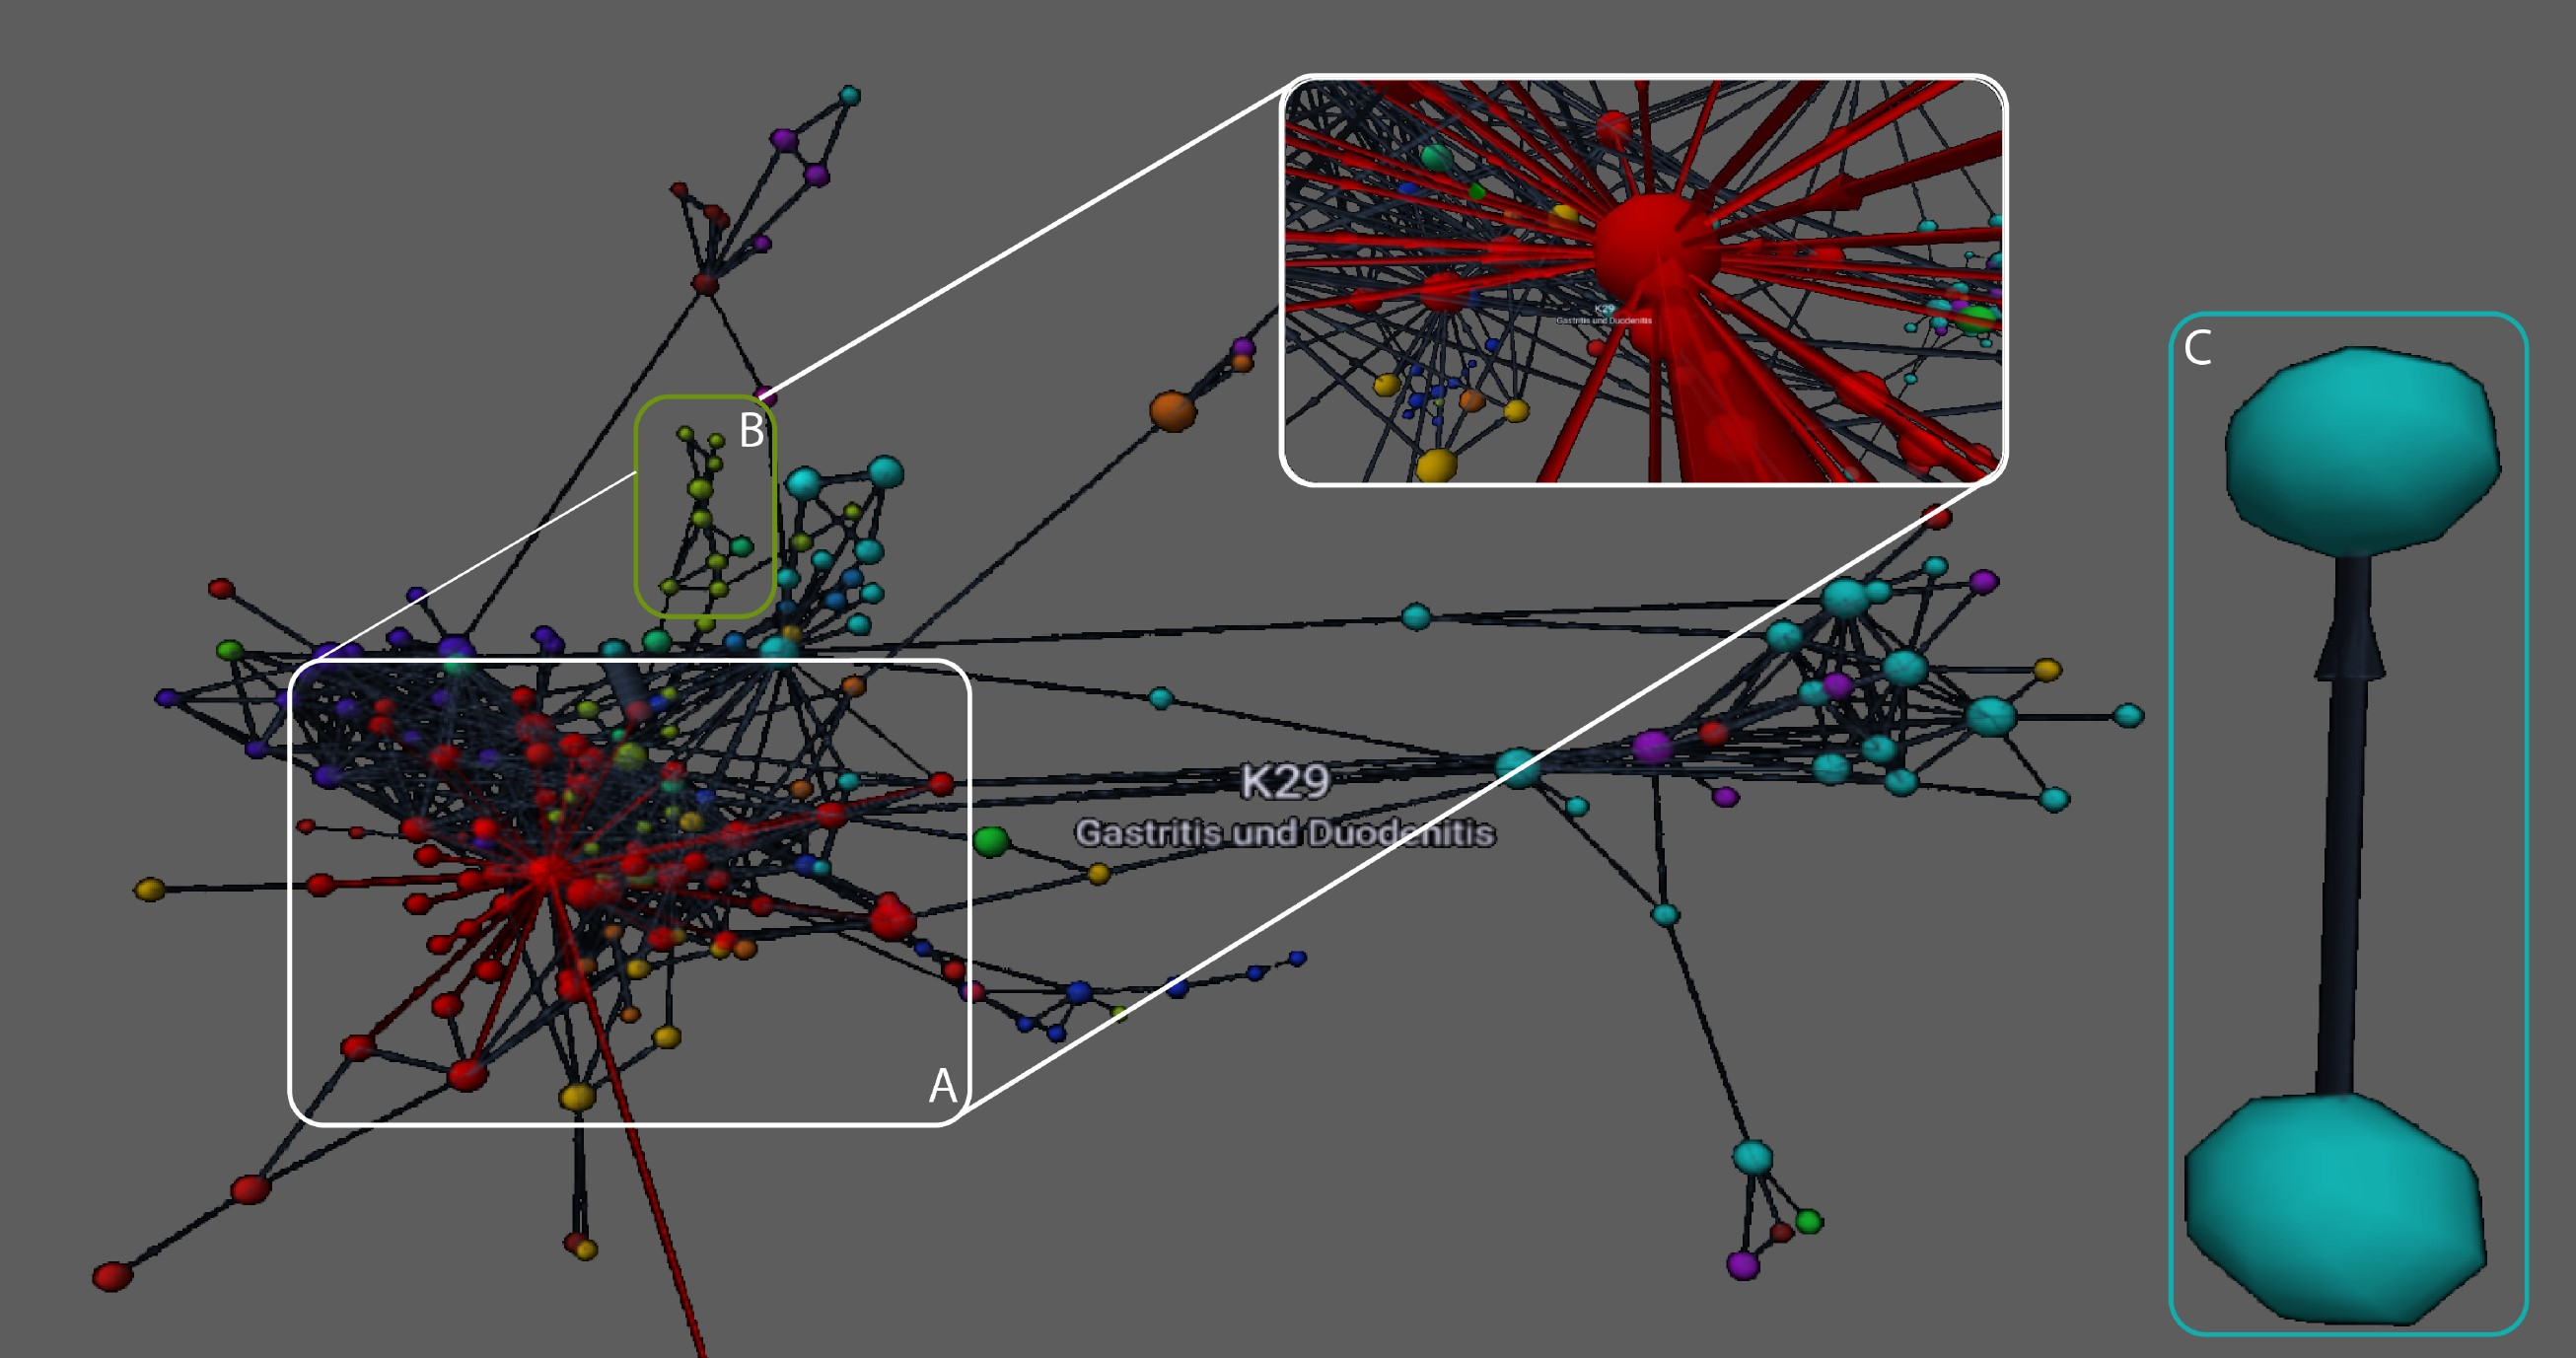
\includegraphics[width=\textwidth]{graphics/screenshotPriorPublication.jpg}
    \caption{Screenshot of the visualization from Sorger et al. \cite{sorger_immersive_2019} we extend our implementation on.}
    \label{fig:priorPublication}
\end{figure}

\section{Technology}

Our application is implemented in plain JavaScript and runs in browsers that support the WebVR standard. 
At the time of writing this applies only to Firefox for Windows, our tested version is 85.0.2 (64-Bit). 
As WebVR is already deprecated and replaced with the new WebXR standard, therefore it is unlikely that other browser vendors will implement the standard in the future.\\
In order to reduce the complexity of the rendering and using the WebVR standard the application uses the framework A-Frame \cite{aframe}. A-Frame internally uses three.js \cite{threejs} as a render engine. The code from the publication we extended uses A-Frame in version 0.9.2 from September 2019, this version uses three.js version 0.108.0. 
The old version of A-Frame brings the limitation of only supporting WebVR because WebXR was not yet ready back in 2019. 
Updating A-Frame to a current version that supports WebXR was not possible within a reasonable time therefore we decided to stick to the old version and only supporting WebVR browsers and headsets.
The primary VR headset we are targeting with our application is the original HTC Vive.

\section{Application Overview}

\subsection{Data Structure}

Listing \ref{lst:internalJSON} shows a minimalistic example of our data structure that we use an input data source. The data is formatted as a JSON object with a flat list of nodes and link. The hierarchical information is encoded with the attributes childNodesIDs and parentNodeID as references. 
In addition to the necessary attributes, each node and link object can have additional attributes depending on the specific dataset.

\begin{lstlisting}[language=json,label={lst:internalJSON},caption=minimal JSON input data structure]
{
    "nodes": [
        {
            "id": "0.0",
            "weight": 4.5,
            "color": "rgb(77, 175, 74)",
            "layer": "0",
            "desc": "0.0",
            "childNodeIDs": [
                "1.1",
                "1.3",
                ...
            ]
        },
        ...
        {
            "id": "1.1",
            "weight": 1.7,
            "color": "rgb(250, 250, 110)",
            "layer": "1",
            "desc": "1.1",
            "parentNodeID": "0.0",
            "childNodeIDs": [
                "2.1",
                ...
            ]
        },
        ...
    ],
    "links": [
        {
            "color": "rgb(77, 175, 74)",
            "layer": "0",
            "source": "0.0",
            "target": "0.1",
            "label": "0.0 - 0.1",
            "linkwidth": 0.35
        },
        ...
    ]
}
\end{lstlisting}

\subsection{Program Flow}
\label{section:programFlow}
\begin{figure}[h]
    \centering
    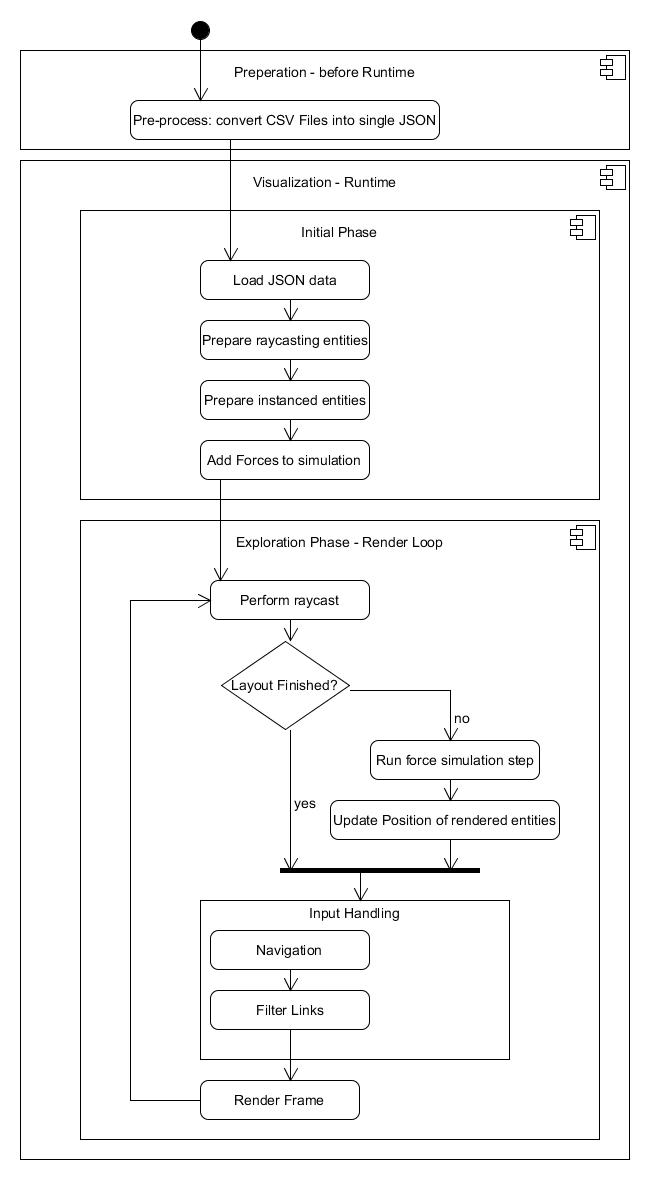
\includegraphics[width=0.74\textwidth]{graphics/vrgraph_flow.jpg}
    \caption{Sequence diagram of the program flow for our application.}
    \label{fig:impl_programFlow}
\end{figure}

To better understand the structure of our application please look at Figure \ref{fig:impl_programFlow}, this describes the program flow and all abstract steps that are necessary for the visualization to work.
A rough separation can be made between the offline preparation phase where the graph data is converted once to our internal JSON data structure (see Section \ref{sec:preprocessing}) and the runtime phase which is executed every time the browser loads the webpage.
After loading the data preparations for the instanced rendering (see Section \ref{sec:rendering}) and the force based layout (see Section \ref{sec:layoutCalculation}) are done.
Then the main render loop is executed which produced a rendered frame for each interaction. In addition, it handles the layout calculation (see Section \ref{sec:layoutCalculation}), navigation and interaction methods (see Section \ref{sec:vrInteractions}), scaling (see Section \ref{sec:scaling}), filtering the graph's links (see Section \ref{sec:linkFiltering}) and performing the ray casting for the virtual laser pointer.
Details on how the ray casting is working is not described in this thesis because we did not adapt this from the original implementation. We only access the objects that got intersected by the virtual laser pointer in other parts such as navigation and interaction. 

\subsection{Virtual Scene Graph}
A Frame Virtual Scene Graph, 

2 Virtual Object Arrays
Raycasting Objects
Rendered Objects

\section{Application Details}

\subsection{Preprocessing Scripts}
\label{sec:preprocessing}


Flexible transforming any CSV Data to our own data format \\
generation of test data \\
coloring, filtering, ... parameter \\
File Format of final processed .JSON for the actual web-based visualization \\

\subsection{Layout calculation}
\label{sec:layoutCalculation}
Implementation Details of Forces, \\
Optimization for Saving Pos and set after done

\subsection{Rendering}
\label{sec:rendering}
Goal of Rendering: 
Performance, Support Transparency of nodes. 

Instancing per Links, 
Instancing per Hierarchical Layer of nodes, 
Transparency,
Wireframe

\subsection{VR Interactions}
\label{sec:vrInteractions}

Camera Rig vs Camera
camera rotation, correct position 
\\
extend controller
\\
Teleport => calculation of target Position (+Grafik?)
\\
FreeFly

\subsection{Scale}
\label{sec:scaling}

Move + Scale\\
Animation
\\

\subsection{LinkFiltering}
\label{sec:linkFiltering}

Filtering of Links\\
Algorithmus multilayer detail layout\\
